\chapter{Coupled models}
\section{Coupled water and heat flow}
\subsection{Goal and Complexity}
\subsection*{Complexity: Medium}

\subsection*{Prerequisites: Heat and Water Flow} 

The goal of this tutorial is to get familiar with the idea of coupled models in 1D. For this we couple the $DRUtES$ standard Richards equation module and the heat module. We apply solar radiation data and rain and evaporation data as input.

\begin{figure}[!h]
\centering
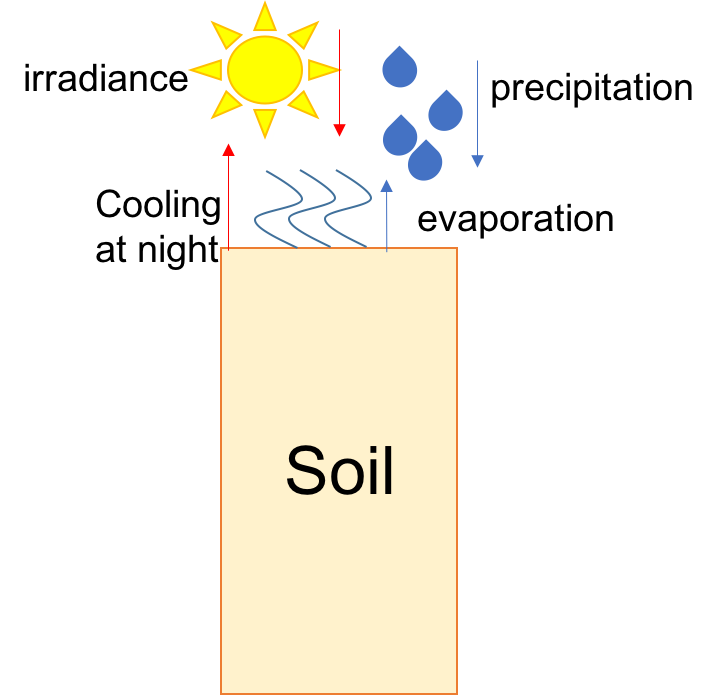
\includegraphics[width=8cm]{Fig_coupledheat/coupled.png}
\caption{Simplified scheme of coupled model.}
\end{figure}

In the real world many coupled processes occur. In our model, heat conduction is dependent on the water flow as it transports the heat in the soil. 
In reality, heat and water is even more closely coupled as soil hydraulic properties are also dependent on temperature, e.g. surface tension and density change with temperature.  

In this tutorial three configuration files will be modified step by step. All configuration files are located in the folder \emph{drutes.conf} and respective subfolders. \begin{enumerate}
\item For selection of the module, dimension and time information we require \emph{global.conf}.  \emph{global.conf} is located in \emph{drutes.conf / global.conf}. 
\item To define the mesh or spatial discretization in 1D,  we require \emph{drumesh1D.conf}. \emph{drumesh1D.conf} is located in \emph{drutes.conf / mesh / drumesh1D.conf}. 
\item To define the radiation and cooling, we require \emph{heat.conf}. \emph{heat.conf} is located in \emph{drutes.conf /heat/ heat.conf}. 
\item To define the precipitation and evaporation, we require \emph{matrix.conf}. \emph{matrix.conf} is located in \emph{drutes.conf /water.conf/ matrix.conf}. 
\end{enumerate}
$DRUtES$ works with configuration input file with the file extension .conf. Blank lines and lines starting with \# are ignored. The input mentioned in this tutorial therefore needs to be placed one line below the mentioned keyword, unless stated otherwise. 

\newpage
\subsection{Scenarios}

For these coupled scenarios we need to define four boundary conditions, two for the heat flow and two for the water flow. We assume simplifying conditions for the bottom boundary. We assume the groundwater table to be at the bottom boundary. This condition does not change over time. Therefore we assign a constant Dirichlet condition for the water flow. We also assume that the temperature of the groundwater remains constant for the given simulation time. This means that we know the temperature, the solution of the heat flow equation and therefore assign a Dirichlet condition for the heat flow. 

In the following scenarios, the water flow is determined by evaporation and precipitation, or more generally time-varying rates of water, therefore the top boundary for the water flow is a Neumann condition. The heat flow over the top boundary is determined by radiation by the sun during the day and radiative cooling during the night. This condition can be understood as a Neumann condition. In these scenarios we want to investigate patterns of temperature oscillations.

We use time-varying boundary conditions for the heat and water flow, which need to be read from files. The file meteo\_heat.bc needs to be renamed to 102.bc in the heat folder. The file meteo\_water.bc needs to be renamed to 102.bc in the water.conf folder.

The material properties needed for scenarios are in Tab. \ref{tab_coup1}.
 
\begin{table}[!h]
\centering
\caption{\label{tab_coup1}Material properties needed for scenarios.}
\adjustbox{max height=\dimexpr\textheight-2cm\relax,
           max width=\textwidth}{

\small\begin{tabular}{l l c c }
\hline
Parameter & Description & Soil \\
\hline

$\alpha$ [cm$^{-1}$]& inverse of the air entry value &0.05 \\
 $n$ [-]& shape parameter &2 \\
 $m$ [-]& shape parameter &0.5  \\
  $ \theta_s$ [-]&saturated vol. water content&0.45 \\
  $ \theta_r$ [-]& residual vol. water content&0.05  \\
  $Ss$ [cm$^{-1}$] & specific storage & 0 \\
  $K_s$ [cm d$^{-1}$] & saturated hydraulic conductivity & 100 \\ 
   $c_l$ [Wd cm$^{-3}$ K$^{-1}$ ] & specific heat capacity of soil & 2.545e-5 \\
  $c_w$ [Wd cm$^{-3}$ K$^{-1}$ ] & specific heat capacity of water & 4.843e-5	 \\ 
  $\lambda$ [W cm$^{-1}$ K$^{-1}$] & thermal conductivity & 0.02 \\ 
\hline
\end{tabular}
}
\end{table}


\begin{figure}[!h]
\centering
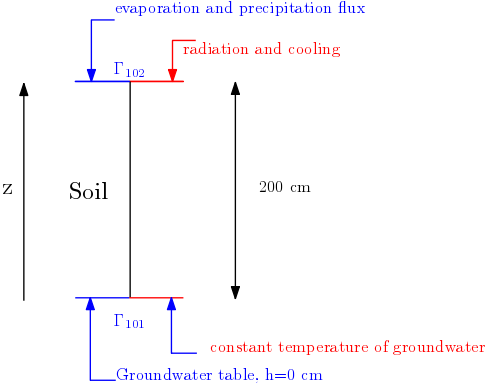
\includegraphics[width=10cm]{Fig_coupledheat/domain_coupled.png}
\caption{1D domain set-up of coupled scenario with top and bottom boundary conditions. There are now two boundary condtions at the top and two boundary conditions at the bottom: heat and water flow. The top boundary is defined by the interactions with the atmosphere and the bottom boundary is defined by the constant groundwater table.}
\end{figure}


\begin{figure}[!h]
\centering
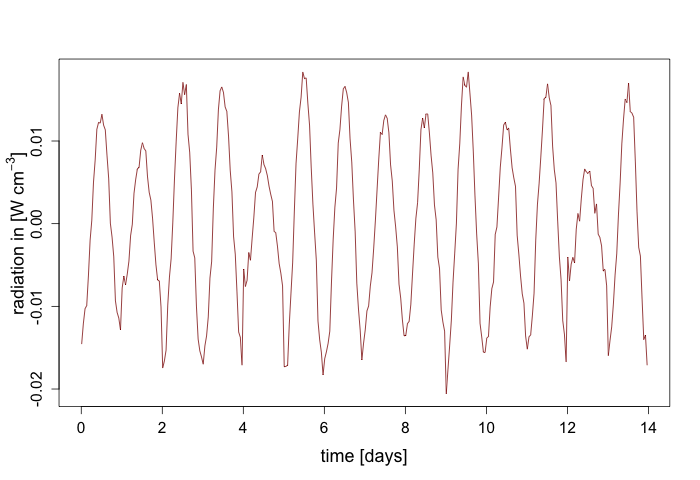
\includegraphics[width=10cm]{Fig_coupledheat/radiation_data.png}
\caption{Heat flow data used for the top boundary}
\end{figure}

\begin{figure}[!h]
\centering
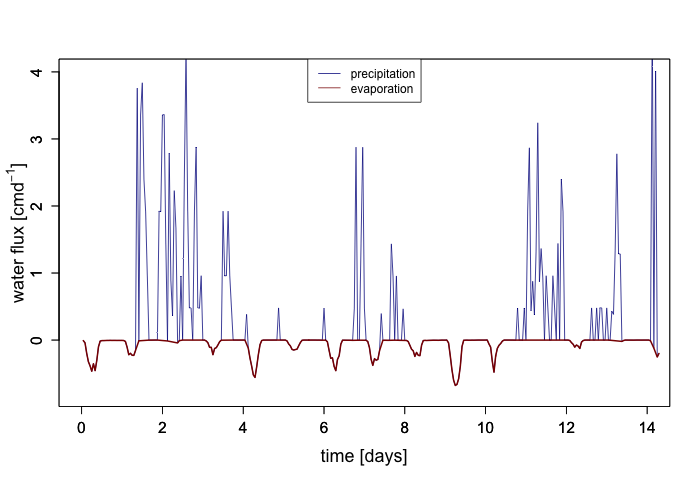
\includegraphics[width=10cm]{Fig_coupledheat/water_data.png}
\caption{Water flow data used for the top boundary}
\end{figure}
\newpage

\section*{Scenario 1}

Coupled model

$global.conf$: Choose correct model, dimension, time discretization and observation times.
\begin{enumerate}
\item Open \textbf{\emph{global.conf}} in a text editor of your choice. 
\item Model type: Your first input is the module. Input is \textbf{heat}.
\item Initial mesh configuration \begin{enumerate}
\item The dimension of our problem is 1. Input: 1.
\item We use the internal mesh generator. Input: 1. 
\end{enumerate}
\item Error criterion \begin{enumerate} 
\item Maximum number of iteration of the Picard method: 20 
\item h tolerance: 1.
\end{enumerate}
\item Time information 
\begin{enumerate} 
%\item integration method is 3 point formula. Input: 30. 
\item Time units are in hours: input d
\item Initial time: 1e-6.
\item End time: 14.
\item Minimum time step: 1e-6.
\item Maximum time step: 0.001.
\end{enumerate}
\item Observation time settings \begin{enumerate}
\item Observation time method: 2
\item Set file format of observation: pure. Output in 1D is always in raw data. Different options will not impact output in 1D.
\item Make sequence of observation time: n
\item Number of observation times: 0
\item Observation time values: \#
\end{enumerate}
\item Observation point settings \begin{enumerate}
\item Number of observation points: 6 
\item Observation point coordinates: 200, 195,180,160,140, 120. Use a new line for each input. \textit{DRUtES} will generate 6 output files, e.g. \textit{obspt\_RE\_matrix-1.out}, where x is the ID of the observation point. 
\end{enumerate}
\item Ignore other settings for now. 
\item Save $global.conf$
\end{enumerate}


$drumesh1D.conf$: Mesh definition, i.e. number of materials and spatial discretization
\begin{enumerate}
\item Open \textbf{\emph{drumesh1D.conf}} in a text editor of your choice. 
\item Geometry information: 200 cm - domain length
\item Amount of intervals: 1
\item
\adjustbox{max height=\dimexpr\textheight-5cm\relax,
           max width=\textwidth}{
\small\begin{tabular}{|c | c | c|}
\hline
density & bottom & top \\
 \hline
4 & 0 & 200\\
\hline
\end{tabular}
}
\item number of materials: 1
\item \adjustbox{max height=\dimexpr\textheight-5cm\relax,
           max width=\textwidth}{
\small\begin{tabular}{|c | c | c|}
\hline
id & bottom & top \\
 \hline
1 & 0 & 200 \\
\hline
\end{tabular}
}
\end{enumerate}

\emph{matrix.conf}: Configuration file for water flow 


\begin{enumerate}
\item Open \emph{matrix.conf} in a text editor of your choice. 
\item How-to use constitutive relations? [integer]: 1
\item Length of interval for precalculating the constitutive functions: 200
\item Discretization step for constituitive function precalculation: 0.1
\item number of soil layers [integer]: 1
\item \adjustbox{max height=\dimexpr\textheight-5cm\relax,
	max width=\textwidth}{
	\small\begin{tabular}{|c | c | c|c | c | c|}
		\hline
		alpha & n & m & theta\_r & theta\_s & specific storage\\
		\hline
		0.05 & 2  & 0.5 & 0.05 & 0.45  &0  \\
		\hline
	\end{tabular}
}
\item The angle of the anisotropy determines the angle of the reference coordinate system. 0 means vertical flow. Anisotropy description. Anisotpropy description and hydraulic conductivity\\ \adjustbox{max height=\dimexpr\textheight-5cm\relax,
	max width=\textwidth}{
	\small\begin{tabular}{|c | c |}
		\hline
		angle [degrees] & K\_11  \\
		\hline
		0 & 100  \\
		\hline
	\end{tabular}
}
\item sink(-) /source (+) term per layer: 0
\item Initial condition is a constant pressure head of -200 cm across the soil.\\ \adjustbox{max height=\dimexpr\textheight-5cm\relax,
	max width=\textwidth}{
	\small\begin{tabular}{|c | c | c|c |}
		\hline
		 init. cond [real] & type of init. cond &RCZA method [y/n] &  RCZA method val.  \\
		\hline
		   0.0           &            H\_tot                      & n		   &          0 \\
		\hline
	\end{tabular}
}
\item number of boundaries: 2
\item \adjustbox{max height=\dimexpr\textheight-5cm\relax,
	max width=\textwidth}{
	\small\begin{tabular}{|c | c | c|c |}
		\hline
		boundary ID& boundary type   & use rain.dat [y/n]   & value  \\
		\hline
	101    &                   1        &           n        &        0.0 \\
	102             &          2         &          y         &       0.0        \\
	
		\hline
	\end{tabular}
}
\item Save matrix.conf.
\end{enumerate}

\emph{heat.conf}: Heat module after Sophocleous (1979). 


\begin{enumerate}
\item Open \emph{heat.conf} in a text editor of your choice. 

\item Couple with Richards equation: y
\item Number of materials or layers: 1 
\item Specific heat capacity of the wall material:  2.545e-5 Wd cm$^{-3}$ K$^{-1}$ 
\item Specific heat capacity of liquid: 4.843e-5  Wd cm$^{-3}$ K$^{-1}$ 
\item Anisotropy: There is no anisotropy. The value is 0.
\item Heat conductivity of the soil material: 0.02 W cm$^{-1}$ K$^{-1}$. 
\item There is NO heat convection of water: 0.
\item The initial temperature is 0$^{\circ}$C across the entire domain: 0.
\item There is no heat source: 0. 
\item We have 2 boundaries at top and bottom of the soil column. We assume a constant temperature of 15 $^{\circ}$C at the bottom where the groundwater table is. We assume the the top to be influenced by radiation and cooling, which are both flux or Neumann conditions. \\
\adjustbox{max height=\dimexpr\textheight-5cm\relax,
           max width=\textwidth}{
\small\begin{tabular}{|c | c | c| c|}
\hline
boundary id & boundary type & use bc.dat & value \\
 \hline
101& 1 & n & 15.0 \\
102& 2 & y & 0.0 \\
\hline
\end{tabular}
}

\item Save heat.conf.
\end{enumerate}

\section*{Run scenario 1}
Run the simulation in the terminal console.
\begin{enumerate}
\item Make sure you are in the right directory. 
\item To execute $DRUtES$: \\
\$ bin/drutes
\item After the simulation finishes, to generate png plots execute provided R script: \\
\$ Rscript drutes.conf/water.conf/waterplots.R -name coupled \\
\$ Rscript drutes.conf/heat/heatplots.R coupled
\item The output of the simulation can be found in the folder out
\end{enumerate}


\section*{Tasks}

\begin{enumerate}
\item Describe the temperature and water content distribution.
\end{enumerate}



\section*{Results}

The water content at the top follows the flux input. The lower the observation point, the less fluctuations can be observed.
The temperature follows the heat flux input. The temperature fluctuations become smaller with depth, but also show a lag time.

\begin{figure}[!h]
\centering
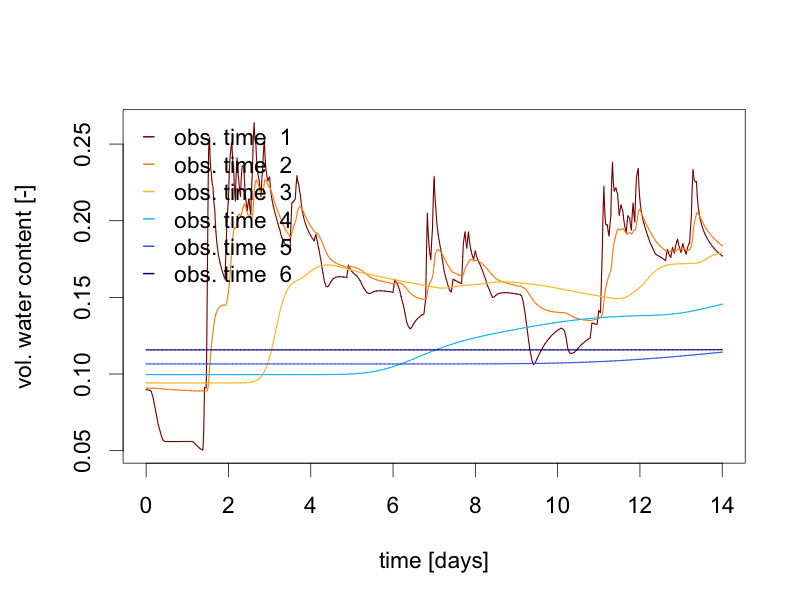
\includegraphics[width=10cm]{Fig_coupledheat/obs_water_point_coupled_standard.png}
\caption{Water content at the observation points}
\end{figure}

\begin{figure}[!h]
\centering
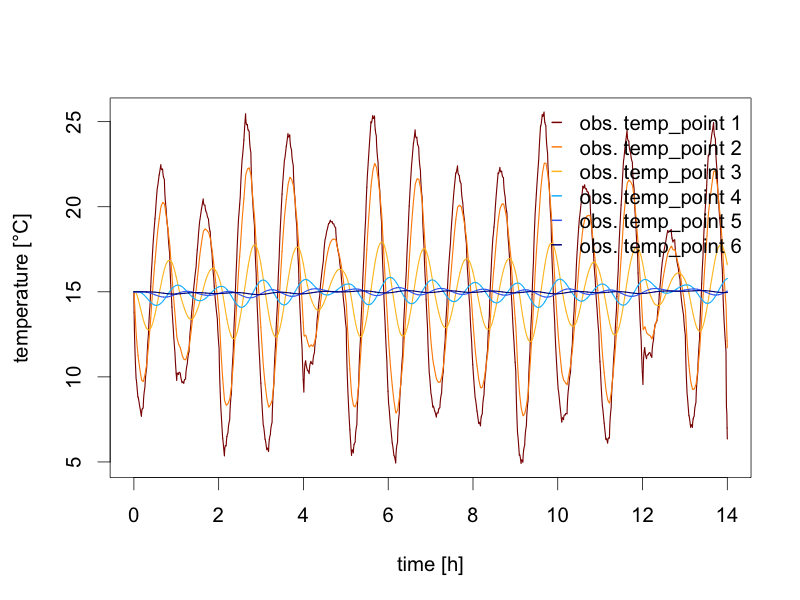
\includegraphics[width=10cm]{Fig_coupledheat/obs_temp_point_temp_coupled_standard.png}
\caption{Temperature at the observation points.}
\end{figure}

\newpage
\newpage

\subsection{Outcome}
\begin{enumerate}
\item You got familiar with the idea of coupled models. 
\item You simulated coupled water flow and heat flow.
\item You understand the influence of distance to input flux and how the top is the most varying layer.
\end{enumerate}
